\documentclass[a4paper, openany]{memoir}

\usepackage[utf8]{inputenc}
\usepackage[T1]{fontenc} 
\usepackage[english]{babel}
\usepackage{amsmath}
\usepackage{amssymb}

\usepackage{booktabs}
\usepackage{fancyhdr}
\usepackage{float}
\usepackage{indentfirst}
\usepackage{graphicx}
\usepackage[linewidth=1pt]{mdframed}
\usepackage{multicol}
\usepackage{fancyvrb}

\pagestyle{fancy}
\fancyhf{}
\fancyhead[LE]{\leftmark}
\fancyhead[RO]{\rightmark}
\fancyhead[RE, LO]{PSD}
\fancyfoot[LE, RO]{\thepage}
\fancyfoot[RE, LO]{Pete Gautam}

\renewcommand{\headrulewidth}{1.5pt}

\chapterstyle{thatcher}
\setcounter{chapter}{13}

\begin{document}
\chapter{Software Architecture}
\section{Component}
There are many definitions of a component in software engineering:
\begin{itemize}
    \item A component is a physical manifestation of an object that has a well-defined interface and a set of implementations for the interface.
    \item A component is a coherent package of software artifacts that can be independently developed and delivered as a unit and can be composed, unchanged, with other components to build something larger.
    \item Components extend object-oriented principles by strengthening the role of the interface and by a separate nation of component specification. Components must conform to a component standard.
\end{itemize}
In general, the notion of a software component refers to a software bundle, a self-contained set of behaviours with well-defined interfaces.

Some components can perform their functions in isolation, but others depend on information and functions provided by other components. A component oriented system is a collection of interacting components that have been combined to realise some wider system purpose.

Components are useful. They allow us to reason about the large-scale subsystems within an overall software architecture. We do not need to worry about the individual behaviour of objects or their implementation in code.

For example, an airline reservation system could be designed as a component oriented system, containing components for:
\begin{itemize}
    \item managing bookings,
    \item taking credit card payments,
    \item issuing boarding passes, 
    \item organising luggage transfer,
\end{itemize}
along with other activities.

The bookings component could probably be used in isolation for other components. Similarly, the credit card processing component might be used by many other systems. An example of such a component is the airline's in-flight drinks cash register.

But, other components such as boarding pass issuer will depend on the booking system. It is not a good idea to issue boarding passes to passengers who haven't paid. Also, luggage management system will depend on the information gathered by the boarding pass issuing component, to know where the luggage will be sent.

\subsection{Components and objects}
There is an overlap between components and objects. They are both software run-time entities and evolving with an address, a state and a behaviour. Moreover, a component has a specification, just like an object has a  class. In a unified modelling language (UML), a component is a specialisation of the object class type, but with a number of distinction characteristics.

A component is a self-contained, self-controlled and evolving bundle of smaller-scale objects. Components are long-lived entities that are generally deployed for the full lifetime of the software system. However, objects are created and destroyed throughout the lifetime. 

A component-oriented system can be distinguished by a middleware framework to mediate interactions between different components. The use of the middleware in a component-oriented system means that the components may be distributed across multiple environments, and even on different hardware systems. The middleware can incorporate an interface definition language (IDL) that is used to define the published interfaces of each component in the system. So, we do not generally interact directly with the component implementation, unlike for an object.

Components are orchestrated by defining an assembly, either during system initialisation or dynamically at run-time. The assembly is distinct from the implementation of components. It specifies which components will satisfy the required dependencies for each component in the system. Normally, a component is identified by a type and a release version.

Components in the same component-oriented system may be implemented in several different programming languages. All of these languages provide support for the same middleware and interface definition language. In addition, each of the interfaces may be provided by a component which is released by a different object within the component.

Loose coupling of a software is generally desirable. So, we could potentially make every object in the system a component to maximise decoupling within the system. This is a bad idea, for the following reasons:
\begin{itemize}
    \item Mediating component interactions through a middleware imposes additional communication costs, on top of that required for direct object-to-object interactions. This is because messages must be encoded, transmitted and decoded by the middleware. For example, consider a JSON RESTful service in the cloud. When a client connects to the RESTful service, it will ask for some JSON data provided by an underlying software component. This component must encode any data into the JSON message, and then transmit it over the network. Finally, the client must decode the JSON content back.
    
    \item There are additional development costs associated with exposing an object as a component. This is because it forms part of the system's published API. The documentation of all the interfaces to a component needs to be maintained. It should be expected that the others will need to understand how to use every component. Also, the interface specifications cannot be readily changed without disrupting the implementation of other components within the system or infrastructure. These might be implemented and maintained by other software teams.
    
    \item The component specification and size should be maintained as part of the system's documentation. If every object in the system is realised as a component, then the system documentation effectively duplicates the underlying language documentation.
\end{itemize}
Decisions about which objects to treat as components will be specific to the software system being developed, to an extent. The role of the software engineer is to decide which are the right objects to the system that should be specified as components that are exposed within the middleware.

\subsection{General purpose and application-specific components}
When building a component-based system, a software engineer will work with two different types of components:
\begin{itemize}
    \item General-purpose components provide common functionality. They are intended to be reused in many applications. For example, a credit-card payment processing component in the reservation system can also be used to collect payments in duty-free shopping at an airport. General-purpose components are normally very well-documented, and stored in some component repository.
    
    \item Application-specific components implement the problem-specific functionality and business logic of the application. For example, a component developed to issue boarding passes at check-in will contain business logic specific to the airline. These components are called the application glue. They orchestrate the behaviour of general-purpose components to realise application-specific needs.
\end{itemize}

Software engineering is very good at developing and maintaining general-purpose components but quite bad at translating code that contains business logic into reusable components. For example, the reservation component could be adapted to other uses, like booking restaurant tables. However, there are often subtle socio-technical reasons why the business logic of a reservation booking system does not translate well into another context.

\subsection{Exposing the right functionalities}
For components they write themselves, a component engineer will need to decide how much of the functionality will be provided by each component under development. Combining lots of functionalities into a component can make the maintenance and the use of the component very complex. This is because changing the component may affect the uses of the component by many other systems. 

Moreover, the interactions between the different component interfaces will also need to be carefully documented. However, making components very simple means that the interaction between the components becomes very complex. Lots of simple component tasks need to be orchestrated to achieve some useful functionality for the application.

One way of mitigating the dilemma is by nesting simpler components within more complex ones. Some of the functionality of the component is encapsulated and replaceable with other sub-components. This approach helps minimise the management of interactions between components at any given level of decomposition of the system.

\section{Component diagrams}
UML component diagrams are a useful way of sketching the high-level architectures of the software system. We express major subsystems as components and the interconnections between them as bound interfaces. 

An example of a UML component diagram is given below.
\begin{figure}[H]
    \centering
    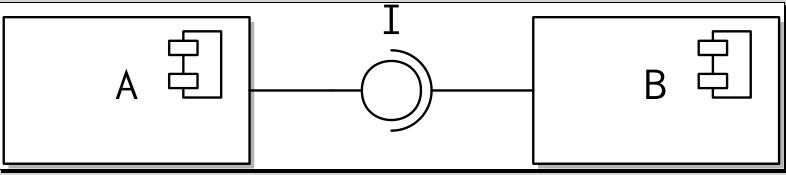
\includegraphics[scale=0.4]{src/14.1 UML Example.png}
    \caption{A UML component diagram}
\end{figure}
\noindent The figure illustrates the basic wiring notation for component diagrams. A component is represented by a box, with a plug widget stereotype. Each component has a label (like A or B). In this example, component A is providing an interface I. This is shown as a facet attached to component A. Component B requires this interface. This is denoted by a connected receptacle drawn around the facet.

We use facets to represent the provision of an interface, and receptacles for the requirement of an interface. This is different to an interface in a programming language, such as Java. An interface on a component is an assembly. It is like a network port on a server. The interface is actively being consumed. The interface is an actual entity with an endpoint address or identifier, like a component. So, if a component is denoted as exposing two interfaces of the same type, they will have different endpoints at run-time.

Next, consider the following UML component diagram.
\begin{figure}[H]
    \centering
    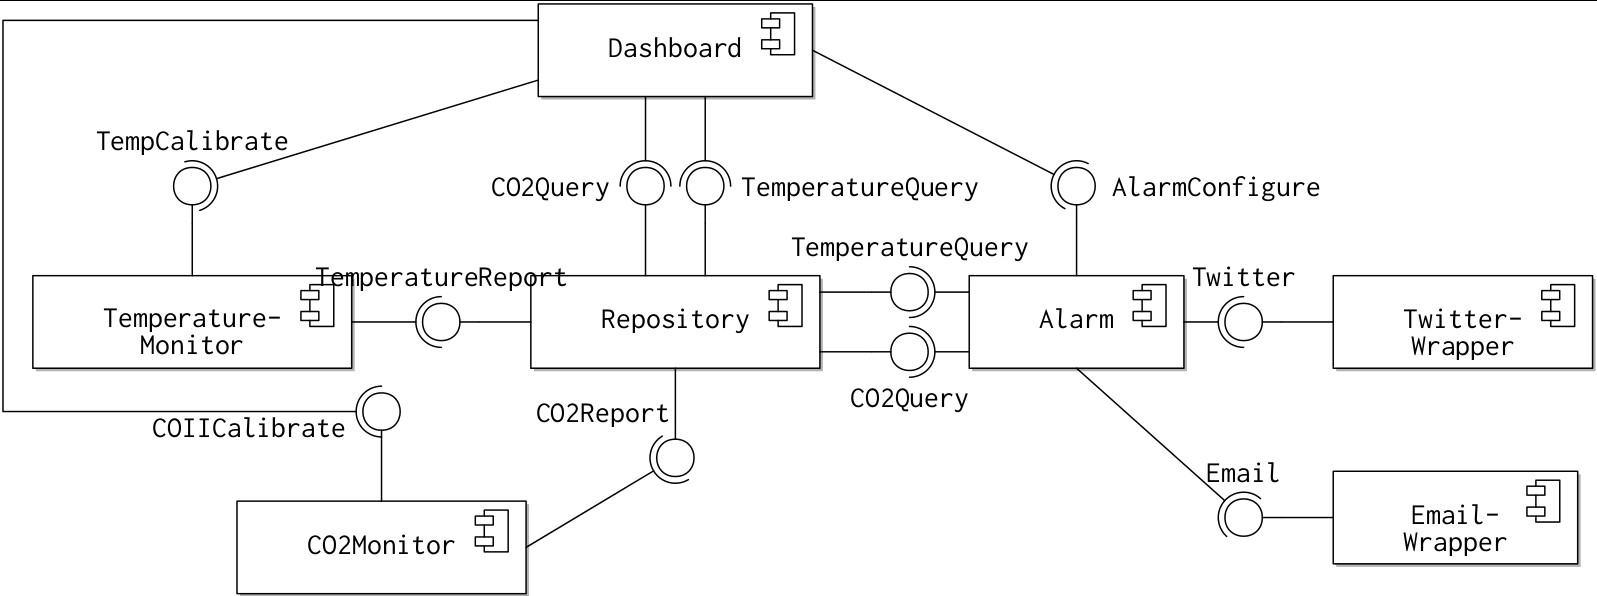
\includegraphics[scale=0.25]{src/14.2 UML Lab monitoring system.png}
    \caption{A UML diagram for a laboratory monitoring system}
\end{figure}
\noindent It denotes a laboratory monitoring system. The system has a number of monitors, such as a CO2 monitor and a temperature monitor. 

A repository component (for storing all the data from sensor monitors) is used to monitor laboratory equipment. The repository provides interfaces to dashboard. The dashboard requires interfaces to different monitor components to be able to configure them. 

There is also an alarm mechanism. This depends on the repository in order to receive information. It can output notifications to different communication system, such as twitter and email.

\section{Separation of concerns}
A key principle in software design is to ensure a separation of concerns. In terms of component implementation, this means that a component should have a clearly defined responsibility for some function(s). It should not be affected by changes to the implementation details of other components.

In a design by contract approach, the interface definition for a component constitutes a contract between the provider and the consumer of some functionality. The interface documentation is called the contract since it should describe the benefits of using the interface that are offered by the providing component. It also states the obligations imposed on the component that proposes to use the interface. The term design by contract describes the process that works with these very precisely documented interfaces to compose software systems.

To provide a contract, the documentation for the interface can include:
\begin{itemize}
    \item the state of the visible component, which is realised by the providing component.
    \item the invariants, which ascribe the legal states of the providing component.
    \item for each operation or method in the interface:
    \begin{itemize}
        \item a signature, which consists of an identifier, an argument identifier and their types, along with the return type of the operation and any exceptions that can be raised as a result of the method being invoked incorrectly.
        \item the pre-conditions, which describe the required state of the providing component before the method can be successfully invoked. It also lists any restrictions on the supplied arguments that cannot be expressed in the signature.
        \item the post-conditions, which describe the state of the providing component after the method invocation has been completed. It also lists any constraints on the values returned to the calling component which cannot be expressed by the interface definition language system.
        \item the semantics, e.g. the correct sequence that the methods should be invoked in, and
        \item the visibility of each operation/method to the other components in the system.
    \end{itemize}
\end{itemize}
An example of a design by contract is given below.
\begin{verbatim}
public 
    @Digits(fraction = 0, integer = 10)
    @Size(min=10,max=10)
String makeCardPayment(
    @Min(value = 0)
Double amount,
    @NotNull
CardType type,
    @Digits(fraction = 0, integer = 16)
    @Size(min=16,max=16)
String number,
    @NotNull
String name,
    @Future
Date expiry,
    @Past
Date begin,
    @Digits(fraction = 0, integer = 4) 
String cardSecurityCode) throws PaymentException;
\end{verbatim}

Different parts of contracts can be expressed in different ways. For example, method signatures are normally expressed formally in an interface definition language, while invariants, pre- and post-conditions (the constraints) and the semantics are documented informally. This might be as source code comments. Nonetheless, it is possible to list them formally. For example, we can make use of the validating package in Java or the OCL constraint language.

In particular, the contract above lists a Java method formally, but we could have equally made use of informal documentation. In practice, less informal documentation may be required if the constraints are expressed formally. 

The method whose contract is shown above processes credit card payments using a specified component interface. The overall behaviour of the method could be described in source code documentation, including a description of each parameter and its constraints. The return value might also be described in source code comments and situations when an exception might be thrown.

These informal constraints expressed in documentation could be strengthened in the method signature, using constraint annotations as shown. The constraints should be consistent with the informal documentation, e.g.
\begin{itemize}
    \item \texttt{@Digits} constraint can be used to indicate that a supplied argument string must be a sequence of digits, of a maximum length.
    \item \texttt{@Future} constraint can be used to state that the date must be at some point in the future.
\end{itemize}

Once specified, the formal constraints can be checked in many ways:
\begin{itemize}
    \item They can be checked statically at compile time.
    \item They can be tested using frameworks, such as JUnit.
    \item They can be checked within the program logic at run-time. For example, we can insert validation checks into the program business logic.
    \item They can be checked by the component middleware at run-time.
\end{itemize}

We might also wonder if it is necessary to have this additional documentation. It certainly reinforces the argument that software engineers should be careful when choosing which objects should be treated as components. This is because the extra overhead of documentation involved is somewhat discouraging. The precise, accurate documentation of an interface is important to prevent the misuse of a component when they are reused in different assemblies.

A good example of poor document specification is the Ariane 5 disaster. A simple casting overflow (64 bit to 16 bit) in the initial reference software was reported to the flight system rather than as diagnostic information. This resulted in the loss of the European space agency \$500 million launch system.

\section{Leaky abstractions}
Another consideration when working with components and their interface is the problem of leaky abstractions. This means that whenever two implementations (provider and requirer of an interface) are wired together in assembly, their evolution is influenced by assumptions by the developers about:
\begin{itemize}
    \item the way that the providing interface will be utilised, and 
    \item the way that the providing interface is realised.
\end{itemize}

It was originally proposed that the leak came from the underlying implementation through the abstraction. The developer of a required component demands to know more about the underlying provider implementation to build a better system. However, the leakage of information goes both ways. This is because the provider of the interface becomes constrained by assumptions on how it is implemented. 

Some argue that every observable implementation detail of the system is part of the contract; not just the interface. For example, assumptions made about the incidental implementation details include:
\begin{itemize}
    \item the ordering of objects received from an iterator over an unordered set. The user should not make any assumptions about which elements should occur first. But, they often make an assumption an ordering based on previous experience. 
    \item the behaviour and the structure of a database system can also leak through the object model interface. For example, knowing how queries will be evaluated can have a big impact on performance.
\end{itemize}

Despite a determination to separate the interface to a component from its implementation, we find that they become coupled. The semantics of a component design become part of the interface. In effect, the distinction between what an interface provides and how it provides the feature is not completely clear cut. Often, how the interface is provided matters to the requirement component.


\end{document}